
%======事務所&代表者紹介======

\clearpage  %ページ途中から続ける場合(Afterwordsの中)はキャンセル

\vspace*{-15mm}   %ページ途中から続ける場合はキャンセル
%\vspace{10mm}   %ページ途中から続ける場合にセット
\hfill
\begin{minipage}[t]{35mm}
%\begin{wrapfigure}[7]{r}{35mm}
%\includegraphics[width=35mm]{profilepic.png}
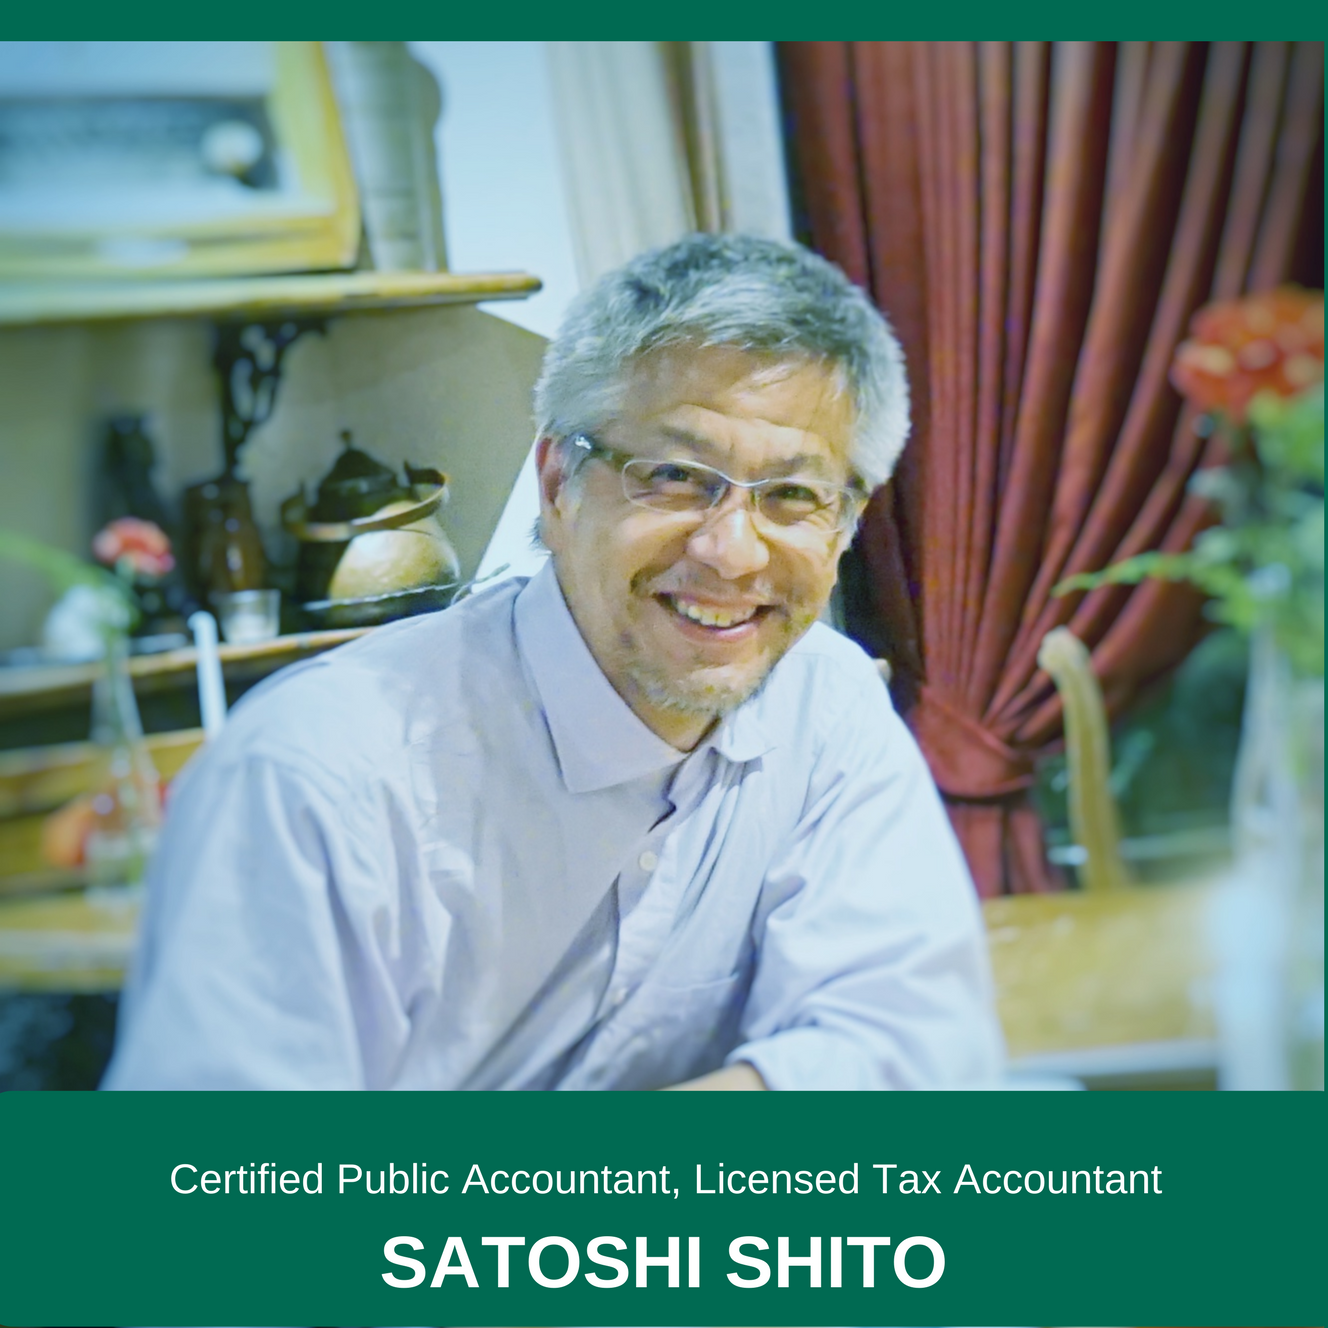
\includegraphics[width=35mm]{shirokanecpa.png}
%\end{wrapfigure}
\end{minipage}

\vspace{-40mm}    %横書き用
\section{My Profile}

\subsection{Personal Information}

\begin{table}[h]
%\begin{spacing}{0.9}
  \begin{tabular}{lll}
Name & {\sffamily \bfseries SATOHSI SHITO} & \\
Professional & \multicolumn{2}{l}{Certified Public Accountant, \textit{1999 (No. 020888)}} \\
\ licenses       & \multicolumn{2}{l}{Certified Tax Accountant, \textit{2013 (No. 127096)}} \\
Affiliation  & \multicolumn{2}{l}{Tokyo Tax Accountant Agency,} \\
 & \multicolumn{2}{l}{Tax Support committee at Shinagawa} \\
         & \multicolumn{2}{l}{Japan CPA Tax committee} \\
         & \multicolumn{2}{l}{Certified Support Agencies for Business Innovation} \\

\includegraphics[width=4mm]{phone.png} & {\sffamily \bfseries +81 80-1257-5877} & \\

\includegraphics[width=4mm]{mail.png} & {\sffamily \bfseries satoshi.shito@shirokanecpafirm.com} & \\

\includegraphics[width=4mm]{website.png} & \multicolumn{2}{l}{\href{https://www.shirokanecpa.com/}{En) https://www.shirokanecpa.com/}} \\
%            & \multicolumn{2}{l}{\href{https://www.shirokanecpafirm.com/}{Jp) https://www.shirokanecpafirm.com/}} \\

\includegraphics[width=4mm]{linkedin.png} & \multicolumn{2}{l}{https://www.linkedin.com/in/satoshishito/} \\    

\includegraphics[width=4mm]{facebook.png} & \multicolumn{2}{l}{Jp)https://www.facebook.com/shirokanecpafirmjp/} \\
            & \multicolumn{2}{l}{En) https://www.facebook.com/Shirokanecpafirm/} \\   
  \end{tabular}
%\end{spacing}
\end{table}

\subsection{Mission}
My objective is to offer adept guidance and steadfast support to entrepreneurs as well as small and medium-sized enterprises. Additionally, I strive to facilitate seamless communication between foreign nationals and the Japanese business community. Rooted in this mission, my commitment lies in nurturing growth and fostering success for all stakeholders as we collectively navigate the path forward into the future.

\subsection{Professional Career Summary}

\subsubsection{M\&A Excellence}
I founded Shirokane CPA Firm on June 25, 2013, in collaboration with esteemed professionals, establishing a boutique consultancy offering specialized financial and tax advisory services. My proficiency spans extensive financial and tax due diligence for Tokyo Stock Exchange-listed entities engaged in M\&A transactions. Moreover, I possess a proven track record in overseeing both statutory and non-statutory audits for discerning clientele.

\subsubsection{Cross-Border Collaboration \& Hong Kong IPO with IFRS}
A significant facet of my journey has centered on nurturing emerging IT venture enterprises, guiding them through intricate tax compliance and strategic business alignment. Leading the audit engagement for Microsoft Japan KK stands as a testament to my leadership. With precision, I directed a dedicated team while concurrently assuming responsibilities as the conduit for Japanese statutory audit, and as a component auditor within Deloitte Seattle's cross-border Microsoft Corp. project. This involvement facilitated seamless collaboration across international boundaries, interfacing with teams in Seattle, Shanghai, and Singapore, fortifying my global perspective on intricate cross-border financial frameworks.

Pioneering noteworthy accomplishments, I orchestrated the groundbreaking Japanese public offering on the Hong Kong Stock Exchange in 2011. Expertly overseeing a Japanese professional team, I meticulously synchronized efforts with the Hong Kong Deloitte team, culminating in the triumphant IPO of SBI Holding, Inc., a prominent force in the Japanese brokerage landscape listed on the Tokyo Stock Exchange.

\subsubsection{Transformation and Strategy in IPO Preparation}
Within Deloitte's Integrated Service Department, I masterminded the metamorphosis of PGM Golf Group in preparation for their Initial Public Offering (IPO). Harnessing my adeptness, I orchestrated strategic transitions and effectively steered the divestiture of credit holdings from Japanese financial institutions. My purview extended to executing post-IPO group audits for a diverse pool of up to 40 companies, and providing strategic counsel on Japan Internal Control Audit intricacies.

My illustrious 19-year CPA career spans partnerships with over 130 diverse companies, evaluating the intricacies of approximately 30 M\&A opportunities. These multifaceted experiences have endowed me with a profound comprehension of varied management paradigms, refining my discernment in critical decision-making, and accentuating the imperative of context-sensitive strategies. From shaping organizational frameworks to orchestrating seamless departmental dynamics and sculpting pragmatic crisis mitigation strategies, I am resolutely prepared to seamlessly integrate my comprehensive expertise and business acumen to surmount future challenges.


%\subsection{Personal Activities}

%{\bfseries \itshape Down-hill Skiing (off-piste):} \\
%From the top of following mountains, \\
%Mt. Fuji (\textit{the highest in Japan, 2012, 2013, and 2014}) \\
%Okuhodaka (\textit{3rd highest in Japan, 2013}) \\
%Harinoki (\textit{2,821m, 2008, 2009}), Tanigawa (\textit{1,977m, 2012-}) \\

%{\bfseries \itshape Traveling:} \\
%California and Oregon, U.S.  (\textit{1991})\\
%Austria (\textit{1998}), Australia (\textit{1998}) \\
%Poland and Estonia (\textit{2015}) \\
%Croatia, Bosnia and Herzegovina, and Montenegro (\textit{2016}) \\
%Domestic area \\
             
%{\bfseries \itshape Scuba Diving:} \\       
%Certification of Advanced Open Water Diver. Experience of \\
%TAKA Dive's 5days cruise  (\textit{1999}) and two 4days diving trips with catamaran yacht at Okinawa, Japan (\textit{2008, 2000}). \\
